\documentclass[a4paper]{report} % estilo do documento

\usepackage[utf8]{inputenc} %encoding do ficheiro
\usepackage[portuges]{babel} % para língua portuguesa
\usepackage{graphicx} % para importar imagens
\usepackage{textcomp}
\usepackage{csquotes}
\usepackage{amssymb}

\begin{document}

\title{Tabuleiros Aleatórios\\ \large{Um relatório sobre os mecanismos de geração de mapas \\ Projeto de LI II.}}

\author{Grupo 74. \\ Gonçalo Faria, José Ferreira e Rui Reis \\ Departamento de Informática \\ Universidade do Minho}
\date{}


\maketitle

\tableofcontents

\chapter{Introdução}

Embora o alvo deste relatório seja esclarecer o funcionamento do nosso algoritmo para criação de tabuleiros aleatórios. Não o faríamos com sucesso sem antes apresentar uma breve explicação de como desenvolvemos o algoritmo para resolver tabuleiros.

O algoritmo de geração de tabuleiros aleatórios é a extensão lógica das ideias desenvolvidas para a encontrar soluções, principalmente porque os tabuleiros gerados podem unicamente conter uma solução.

Os mecanismos e estruturas já desenvolvidas para resolver tabuleiros , foram reformulados por forma a não descartar componentes valiosas que nos permitem extrair mais informação para o processo de geração.

\chapter{Árvore de Soluções}

\section{Funcionamento}

Para representar o espaço de sub tabuleiros válidos introduzimos um grafo que é essencialmente uma árvore binária, no entanto não direcionada, com as seguintes propriedades invariantes:

\begin{enumerate}
    \item \label{itm:first} Cada nó da árvore bifurca em nós que apenas diferem numa determinada posição do tabuleiro. Um dos nós filhos tem nessa posição uma peça cruz e o outro tem uma peça círculo. Tal verifica-se se e só se essa peça nessa posição mantém o tabuleiro válido, caso contrário o nó é a raiz da árvore conjunto vazio (\textit{NULL}). 
    \item \label{itm:second} Para cada nível na árvore está associada uma posição no tabuleiro e o oposto também é verdade, ou seja, para cada posição no tabuleiro só há um nível associado.
    \item \label{itm:third} Se há um caminho que liga a raiz a uma folha então essa folha é necessariamente um solução.
    \item \label{itm:fourth} Para cada tabuleiro com $k$ peças livres existem $k!$ possíveis árvores que podem corretamente representar o seu espaço de sub-tabuleiros válidas, no entanto as folhas e o número de folhas são iguais em todas as diferentes árvores.
\end{enumerate}

As propriedades em cima permitem-nos essencialmente chegar às seguintes conclusões:

\begin{itemize}
    \item Se um nó é a raiz de uma sub árvore desnaturada então o tabuleiro que este representa tem uma única solução.
    \item A árvore que representa um tabuleiro sem solução é o conjunto de vazio. Ou seja, não existe árvore que representa um tabuleiro sem soluções.
\end{itemize}

\newpage

\section{Construção}

O algoritmo para criação da árvore é naturalmente recursivo devido à natureza indutiva do tipo de dados que decidimos usar.

Inicialmente verifica-se se o nó recebido é uma posição válida. Caso seja, é bifurcado e o processo é repetido nos nós recentemente criados. Assim, um tabuleiro é propagado nas chamadas recursivas, por referência, e vai sendo modificado para corresponder ao nó a ser analisado por forma a facilitar as validação.  Assim é possível re-utilizar métodos já criados noutras partes do projeto para a validação deste.

Na eventualidade do nó a ser analisado não corresponder a um tabuleiro válido este é eliminado, pois, por um lado, este certamente não levará a uma solução e, por outro lado, é necessário manter a propriedade invariante em (\ref{itm:third}).

Após a chamada recursiva são consultados os nós filhos gerados. Caso ambos estes sejam o conjunto vazio então significa que embora o nó atual seja válido ele não leva a nenhuma solução logo por (\ref{itm:third}) este tem de ser também eliminado. 

Adicionalmente por razões que se tornarão claras nas secções à frente atribuímos a cada nó uma das 3 categorias, \textbf{\textit{Road, Treasure, Trail}}.

\begin{figure}[h]
    \centering
    \includegraphics[scale=0.2]{tree.png}
    \caption{Representação visual de cada categoria.}
\end{figure}

A categoria de \textit{road} destina-se a nós que não são solução, no entanto podem levar a mais do que uma solução. \textit{Treasure} significa que o nó corresponde a uma solução do tabuleiro. Por fim \textit{trail} significa que o nodo é a raiz de uma árvore desnaturada, ou seja o tabuleiro que este representa tem uma única solução.

Por fim, no nosso algoritmo de geração da árvore não foi indicado o mecanismo de atribuição de posições a cada nível, isto não foi deixado ao acaso, o nosso algoritmo recebe como parâmetro uma função que se encarrega de atribuir a próxima posição a desenvolver.

\chapter{Função de seleção por nível}

A ideia por detrás desta função foi concebida no princípio da realização da resolução de tabuleiros quadrados vazios.

O que nós pensamos foi que a melhor forma de resolver um tabuleiro quadrado de lado $n$, sendo que para tabuleiros vazios e quadrados com os lados maior que 5 têm sempre unicamente 8 soluções temos unicamente que, supondo que temos acesso à resolução dos tabuleiros de lado $n-1$ que descobrir quais são as $2n-1$ peças que faltam para que este este esteja totalmente preenchido e que se mantenha válido.

Esta perspetiva deu-nos a intuição que promover o agrupamento de peças era a melhor forma de descartar várias possibilidades rapidamente, logo a função de atribuição de posições que usamos tenta recriar exatamente este comportamento.

\chapter{Solução do Tabuleiro}

Tendo obtido a árvore que representa espaço de sub-tabuleiros válidos ter-se-á unicamente que a percorrer até se alcançar uma folha. Por razões que se tornarão evidentes, introduzimos uma pequena heurística na seleção do caminho. Quando tendo a opção de seguir dois caminhos, o nó da categoria \textit{trail} tem prioridade. 

\chapter{Geração Aleatória}

\section{Teoria}

Para a geração de mapas, tendo unicamente a dificuldade e o número de linhas e colunas do tabuleiro a gerar em conta, é criado um tabuleiro ‘matéria prima’ que será a raiz da árvore a ser criada.

O tabuleiro matéria prima é o resultado da atribuição de peças bloqueadas aleatoriamente com base numa dada probabilidade.

Tendo o tabuleiro matéria prima criado é gerada, com o algoritmo descrito anteriormente, a árvore deste. Procede-se à seleção de uma das soluções.

Com uma possível solução do tabuleiro matéria prima são testadas todas as peças que o compõem na tentativa de remover todas aquelas que não são necessárias para que o tabuleiro mantenha uma única solução.

O processo de teste é o de essencialmente trocar a peça em questão por vazio e verificar se a árvore que este novo tabuleiro gera contêm como raiz um nó do tipo trail.

A heurística referida para selecionar folhas que dão prioridade a seleção de sub árvores que têm uma única solução é usado na tentativa de assegurar que o tabuleiro final resultante deste processo é um que contêm um elevado número de peças vazias.

Tendo havido a necessidade de aceder a árvore deste tabuleiro final para consultar se contêm uma única solução. Esta é aproveitada para recolher todas as peças que a compõe a sua solução final.

Por fim, são selecionadas aleatoriamente algumas das peças que compõem a solução e acrescentadas ao tabuleiro.

\section{Dificuldade de diferentes tabuleiros}

As duas dificuldade requeridas no enunciado são obtidas no caso do mapa fácil obtendo uma probabilidade de $4\%$ de uma dada peça ser bloco e no caso de díficil $11\%$ assim como a quantidade de peças que se mantêm vazias sendo a percentagem no caso fácil de $40\%$ e $30\%$ do difícil.

\section{Resultados}

\subsection{Dificuldade Fácil}

\begin{figure}[ht]
    \centering
    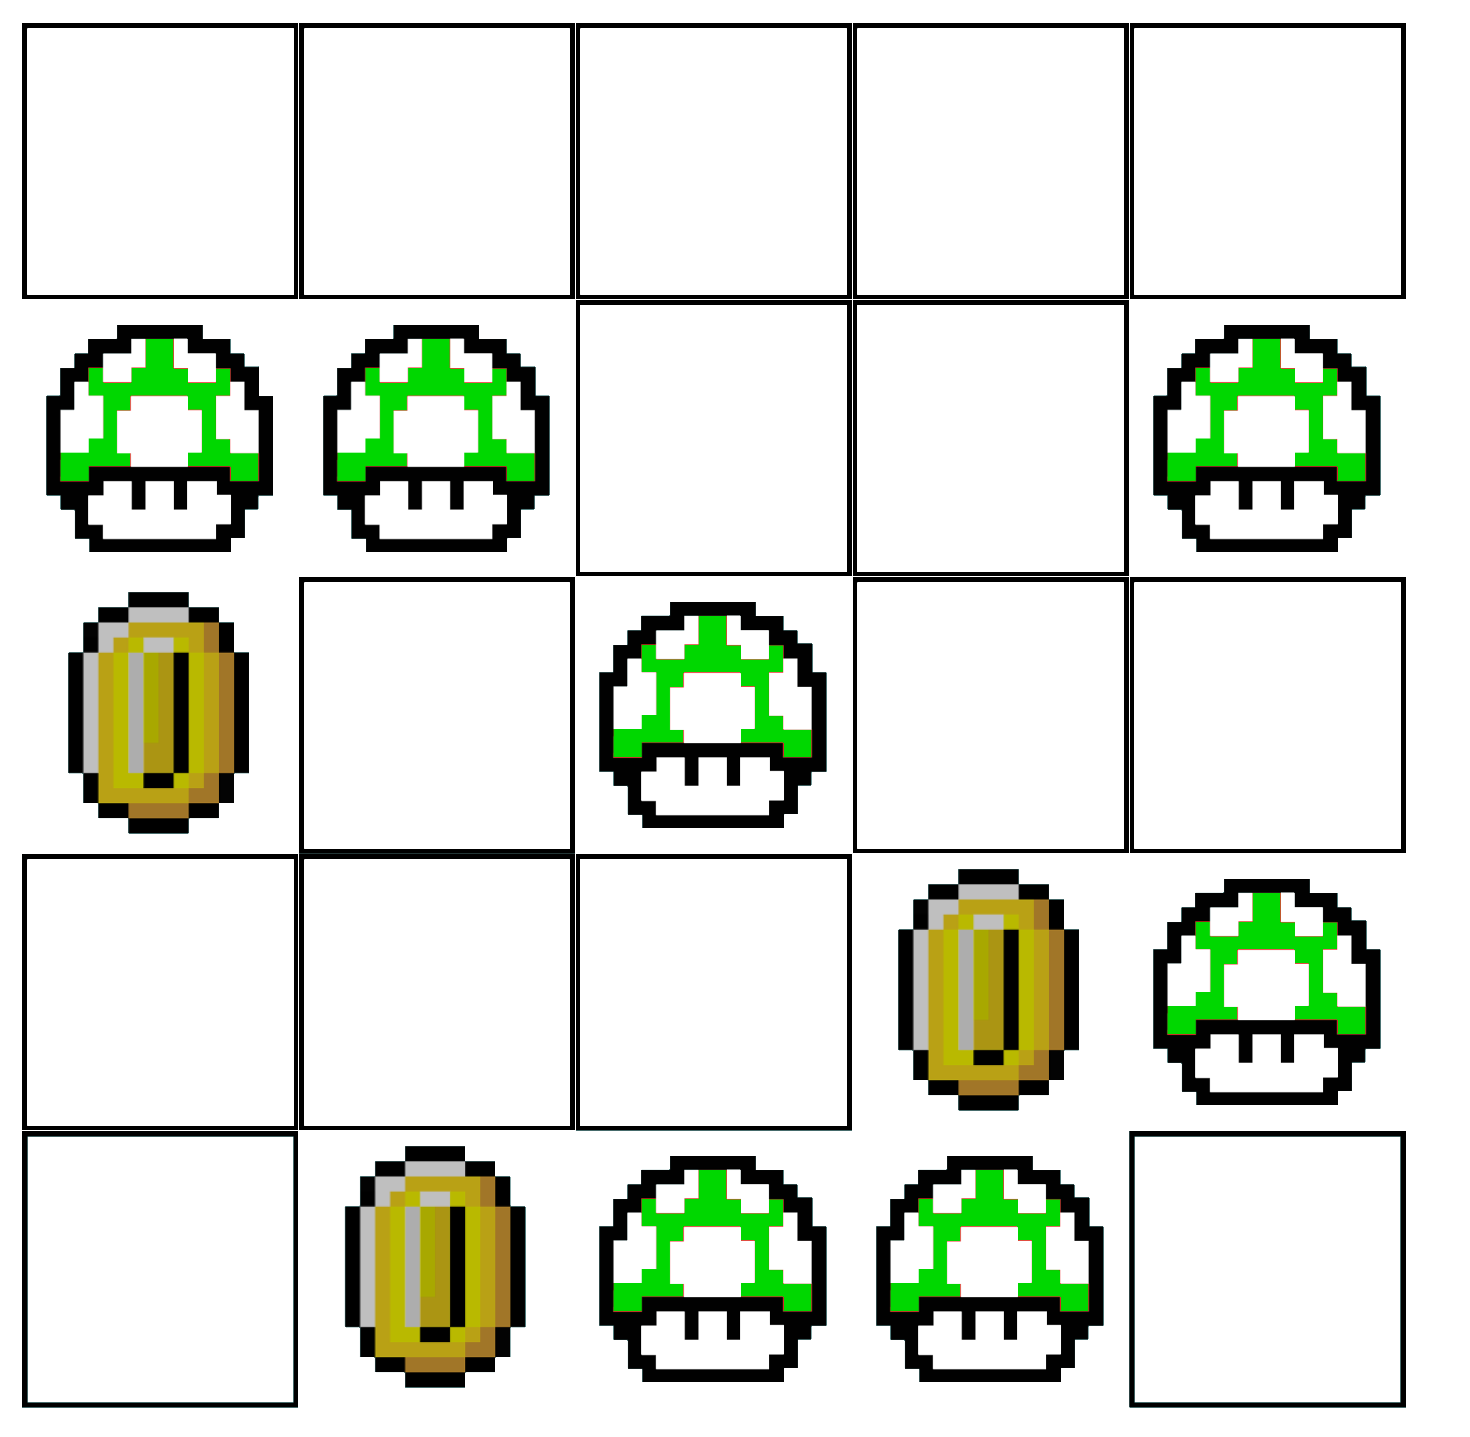
\includegraphics[scale=0.25]{1_5_5.png}
    \caption{Mapa gerado com dificuldade fácil.}
\end{figure}

\begin{figure}[ht]
    \centering
    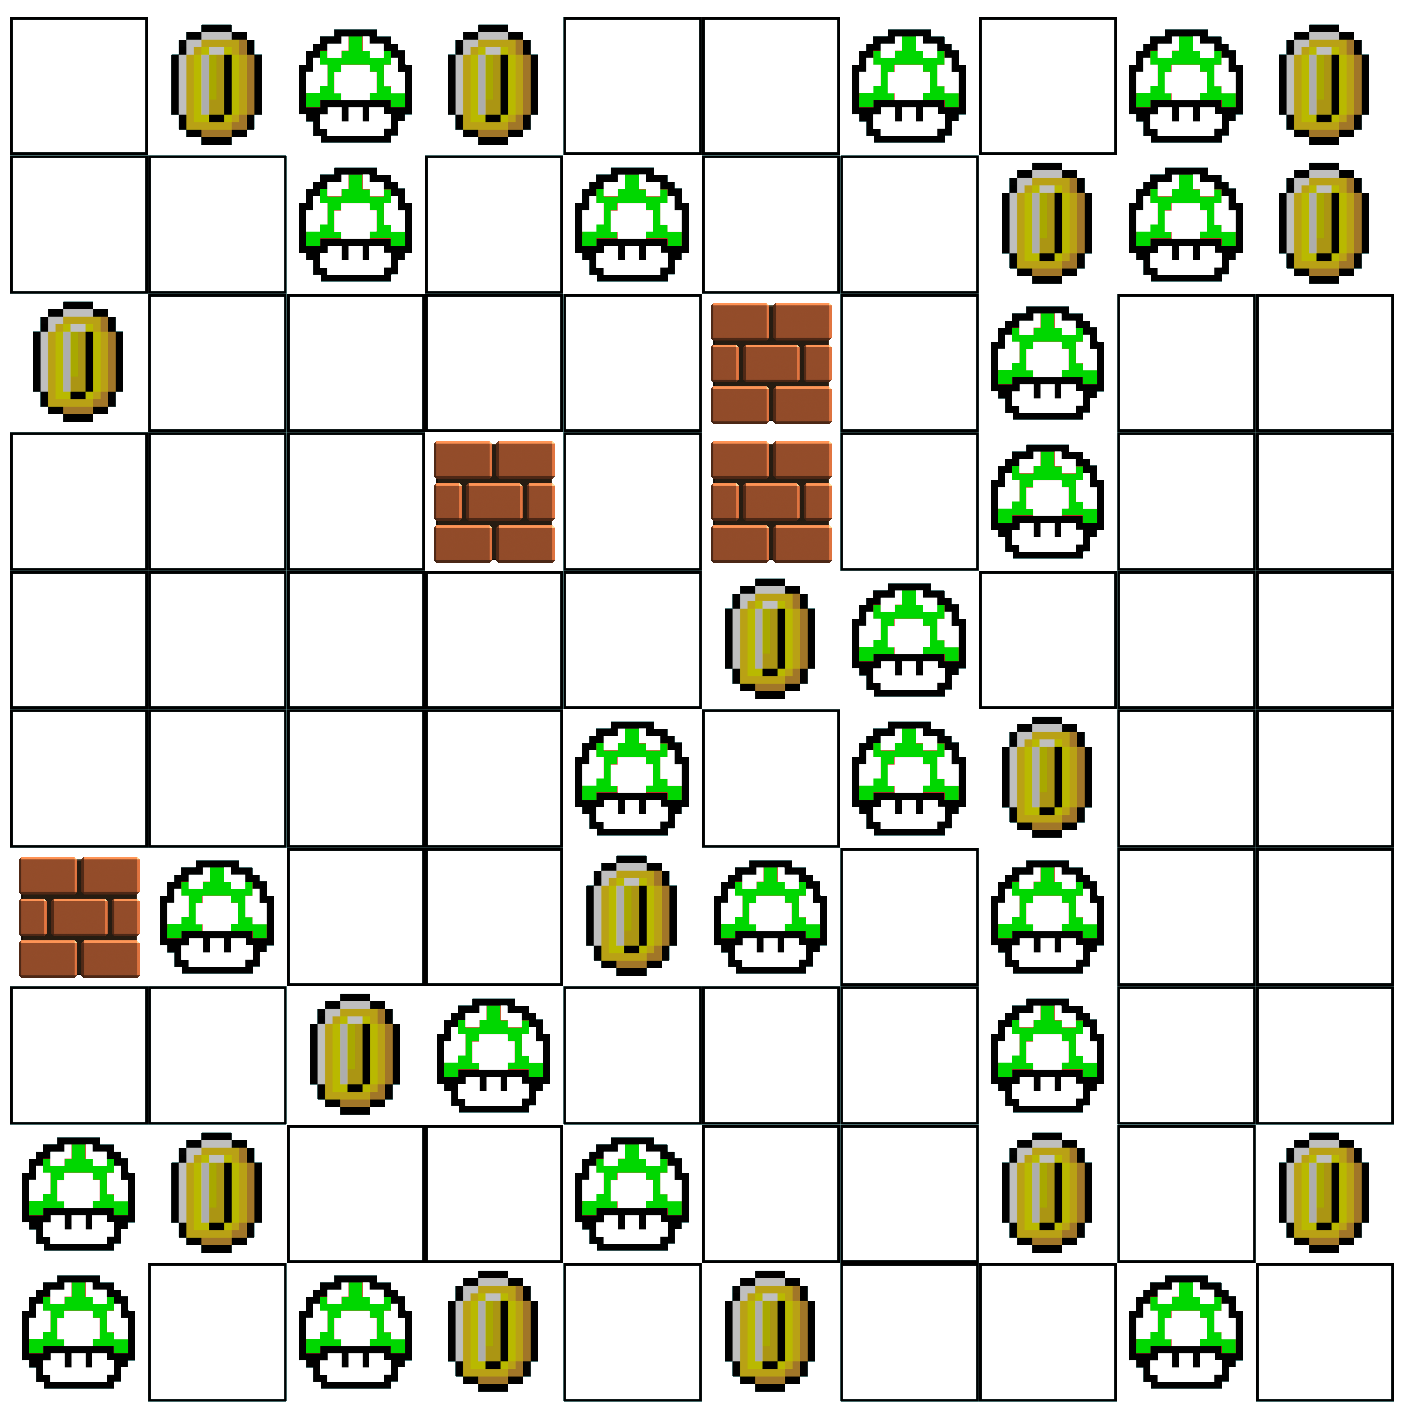
\includegraphics[scale=0.25]{1_10_10.png}
    \caption{Mapa gerado com dificuldade fácil.}
\end{figure}

\newpage

\subsection{Dificuldade Difícil}

\begin{figure}[ht]
    \centering
    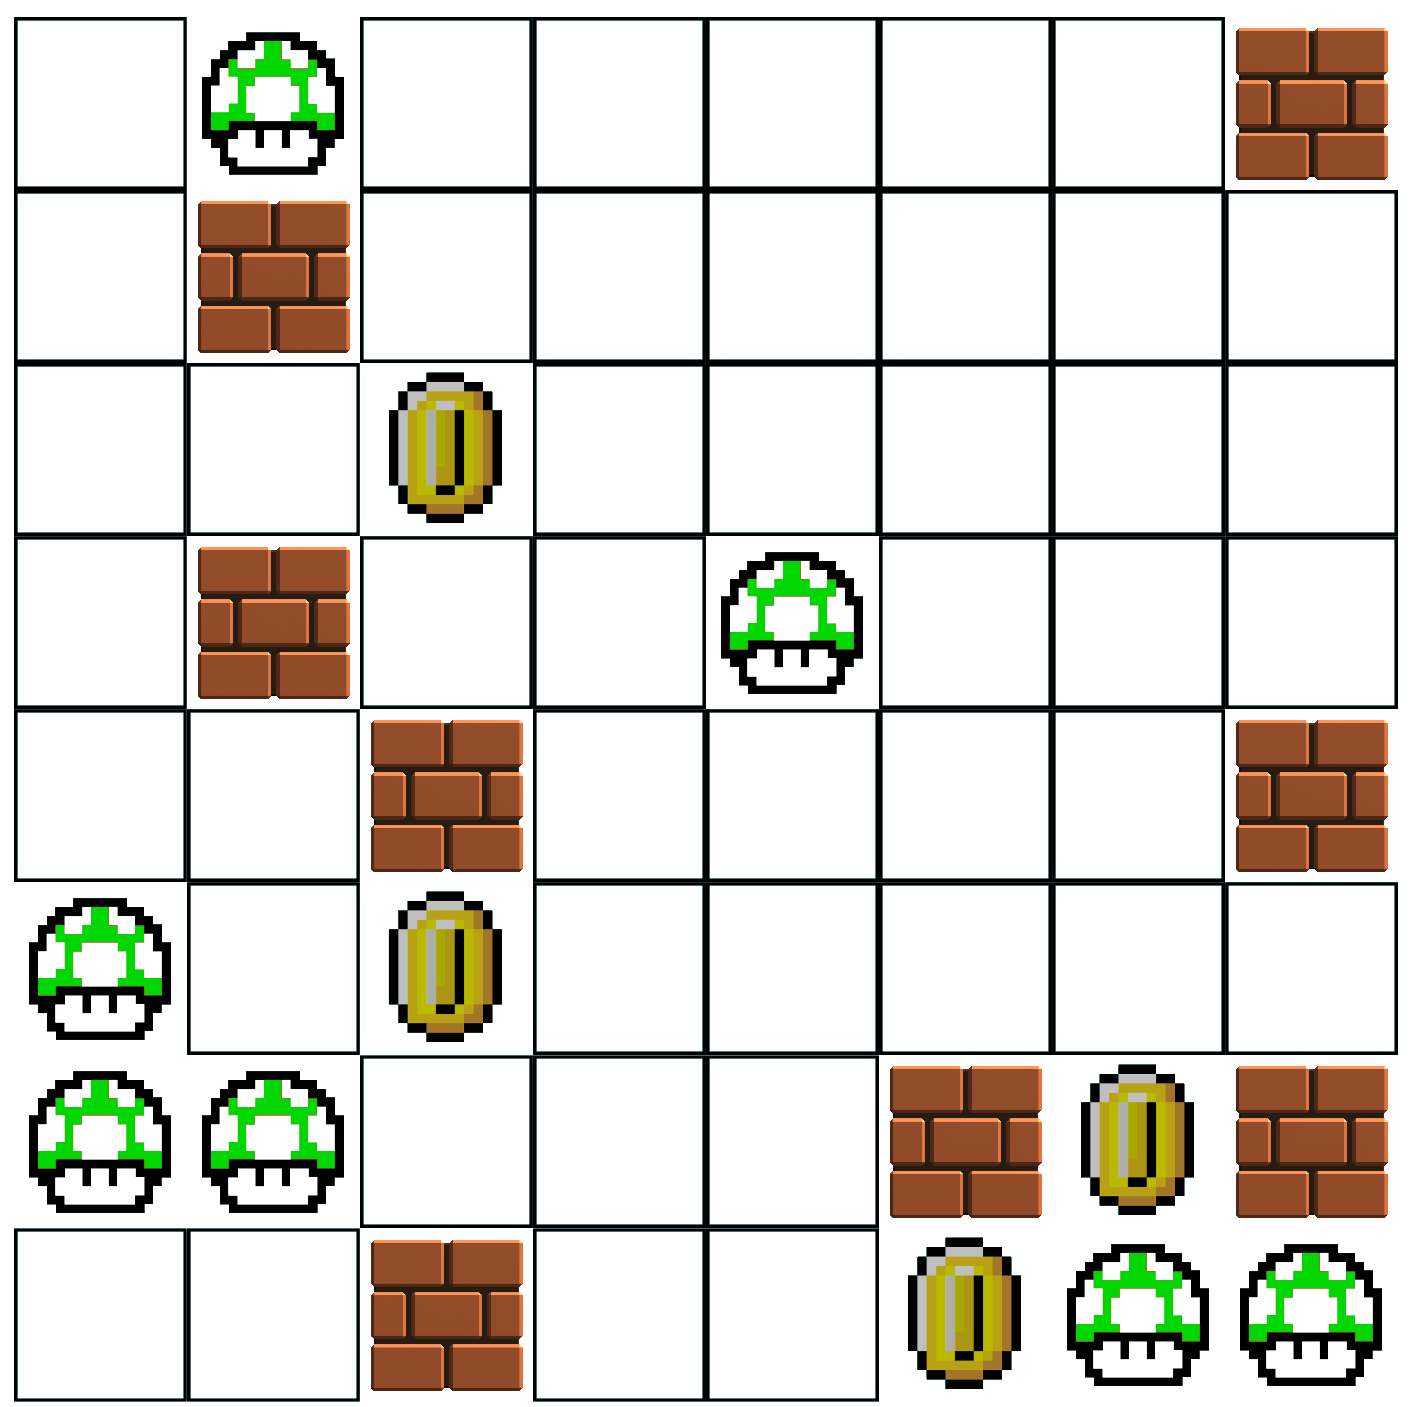
\includegraphics[scale=0.25]{2_8_8.png}
    \caption{Mapa gerado com dificuldade difícil.}
\end{figure}

\begin{figure}[ht]
    \centering
    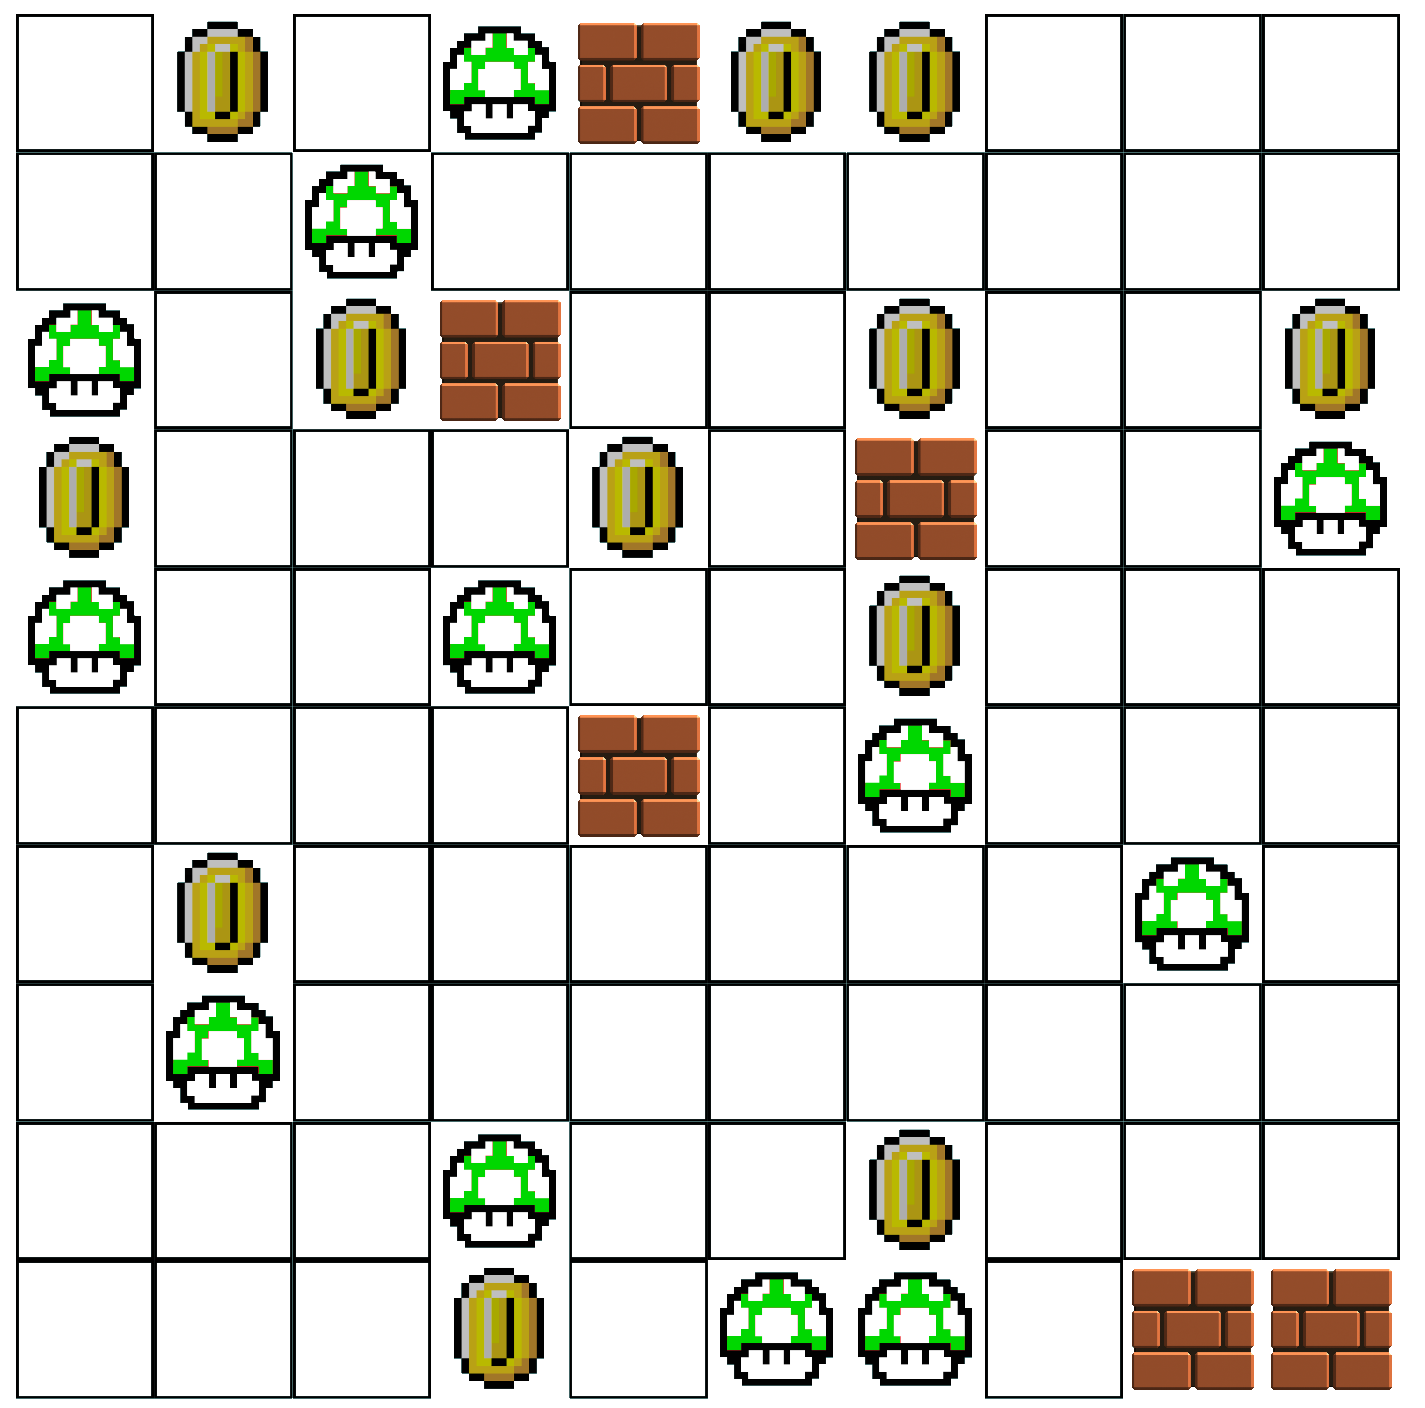
\includegraphics[scale=0.25]{2_10_10.png}
    \caption{Mapa gerado com dificuldade difícil.}
\end{figure}

\end{document}
